\documentclass[a4paper,12pt]{report}

%\usepackage[utf8x]{inputenc}
%\usepackage[T1]{fontenc}
\usepackage{lmodern} % For changing the font
%\usepackage{subcaption}

\usepackage{graphicx} % For including images
\usepackage{wrapfig} % For using images wrapped inside some text
\usepackage{hyperref} % For adding hyper reference links
%\usepackage{float} % The float package provides the H option to floating environments, which completely stops them from floating.

% \PrerenderUnicode{é} % This is for fixing the issue or having index/header 'é' error

\hypersetup{
pdftitle={A Decentralized electronic election system based on blockchain technology.},
pdfsubject={Graduation thesis},
pdfauthor={Rahmouni Abdelhak},
pdfkeywords={Blockchain, Decentralization, Electronic electoral system, Electronic voting}
}

%		Header		%		
\usepackage{fancyhdr}
\pagestyle{fancy}
\rhead{\thepage}
\lhead{\leftmark}

\usepackage{makeidx}
\makeindex
\usepackage[toc,acronym]{glossaries}

\makeglossaries
 
\newglossaryentry{cryptocurrency}
{
    name=cryptocurrency,
    description={A cryptocurrency, crypto-currency, or crypto is a digital asset designed to work as a medium of exchange wherein individual coin ownership records are stored in a ledger existing in a form of a computerized database using strong cryptography to secure transaction records.}
}
\newacronym{EVM}{EVM}{Ethereum Virtual Machine}

\begin{document}

%\input{Parts/remerciements.tex}
%\input{Parts/resume.tex}

\tableofcontents
\listoffigures
%\listoftables --- until now I haven't used any tables
\printindex
\printglossary[type=\acronymtype]
\printglossary

\newpage

\thispagestyle{empty}

\vspace*{2cm}

\begin{center}
\textbf{Abstract}
\end{center}

%Apart from being the backbone of the cryptocurrencies of the world, blockchain technoloy enthusiastes believe that crypto is only a fraction of what the blockchain will eventually yield to our future societies.\medskip

This research aims to explore one very promiment and potential application for the blockchain, which is a decentralized electronic voting system, by creating a proof-of-concept of a voting application, capable of launching an election, casting votes and displaying results, all while ensuring transaprency, anonymity, security and above all the correctness of the results.\medskip

%Throughout the research both advantages and incoviniences and even research avenues encountered will be highlighted, for essentially the purpose of this research is to gauge to what degree the blockchain is an appropriate solution for a voting system\bigskip

\textbf{Keywords:} Decentralized Electronic Voting System, Voting, Blockchain

\chapter{Introduction}

Since the dawn of democracy, elections have been accused for the lack of transparency and security. As societies all over the world are rapidly adopting technology across all aspects of society, a digitalized democratic system of voting might just be the next evolutionary step towards a transparent and trusted electoral system.

In this first chapter, we introduce our work on proposing a decentralized voting system.

\section{Background}

As the hype surrounding bitcoin\cite{satoshinakamotoBitcoinPeertoPeerElectronic} is slowly waning, the industry is becoming more and more interested in its underlying technology: the Blockchain. Now, proponents claim Blockchain technology to be one of the most important new technologies of our time, about to take society by storm, and bitcoin served as the first, most thorough and complete proof of concept. In fact, Marc Andreessen, founder of VC firm Andreessen Horowitz and one of the most influential members of Silicon Valley, claimed in a New York Times article that the invention of the Blockchain is as important and influential as the creation of the Internet itself\cite{andreessenWhyBitcoinMatters1390323270}.\smallskip

Along with assets registry, secure sharing of medical data and supply chain and logistics monitoring, electronic voting is one of the most prominent potential applications for the surging Blockchain technology.

\section{Key Concepts}

Our work revolved around few key concepts, the most critical of them all are introduced in the subsequent sections.

\subsection{Voting}

According to Oxford English dictionary, voting (also known as election) is \textit{"a formal indication of a choice between two or more candidates or courses of action, expressed typically through a ballot or a show of hands"}, and the very first forms of voting date back to approximately 508 B.C in ancient Greece where the earliest form of democracy was implemented\cite{mikehoganHistoryElectionsOnline}. Greeks had a "negative" election -- that is, each year voters, who were the male landowners, were asked to vote for the political leader or "candidates" they most wanted to be exiled for the next ten years.

The early ballot system was voters wrote their choice on broken pieces of pots, ostraka in Greek, and from this name comes our present word to ostracize. If any "candidate" received more than 6,000 votes then the one with the largest number was exiled. If no politician received 6,000 votes then they all remained. Since voters were only male landowners, the number of voters was small. If there was a fairly even spread of votes, no one would be exiled, so usually, only very unpopular political leaders were ostracized or exiled.\cite{mikehoganHistoryElectionsOnline}

The election is the backbone of modern democratic societies, it often takes place at a polling station; it is voluntary in some countries, compulsory in others, such as Australia\cite{australiangovernmentCOMMONWEALTHELECTORALACT}.

\subsection{Electronic voting}

Electronic voting (e-voting) is a security-critical application of electronic democracy (e-democracy). E-voting has become an applicable alternative for many non-governmental elections recently. There are a number of e-voting experiments currently being employed by various countries in political area as well. However many discussions, controversies and irregularities have been raised about them. The e-voting experience in Ohio in 2004 is one of the well-known examples which caused many discussions about vote miscount and modification. Therefore, it is not easy to say that an accurate and faultless e-voting is likely to become viable soon for governmental elections\cite{orhancetinkayaVerificationValidationIssues}.

E-voting is an inter-disciplinary subject and should be studied together with the experts of different domains, such as software engineering, cryptography, politics, law, economics and social sciences. Although many people have worked on this subject, mostly e-voting is known as a challenging topic in cryptography. The challenge arises primarily from the need to achieve voter anonymity, in other words to remove voter’s identity from his cast ballot in order to ensure voter privacy whereas ensuring the e-voting has been done correctly without any violation and ensuring only eligible voters’ votes have been counted. Thus, e-voting has been intensively studied in the last decades\cite{orhancetinkayaVerificationValidationIssues}.

\subsection{Blockchain technology}

A Blockchain is essentially a distributed database of records, or public ledger of all transactions or digital events that have been executed and shared among participating parties. Each transaction in the public ledger is verified by consensus of a majority of the participants in the system. Once entered, information can never be erased. The Blockchain contains a certain and verifiable record of every single transaction ever made\cite{michaelcrosbyBlockchainTechnologyBitcoin2016}.

\begin{figure}[h]
	\centering
		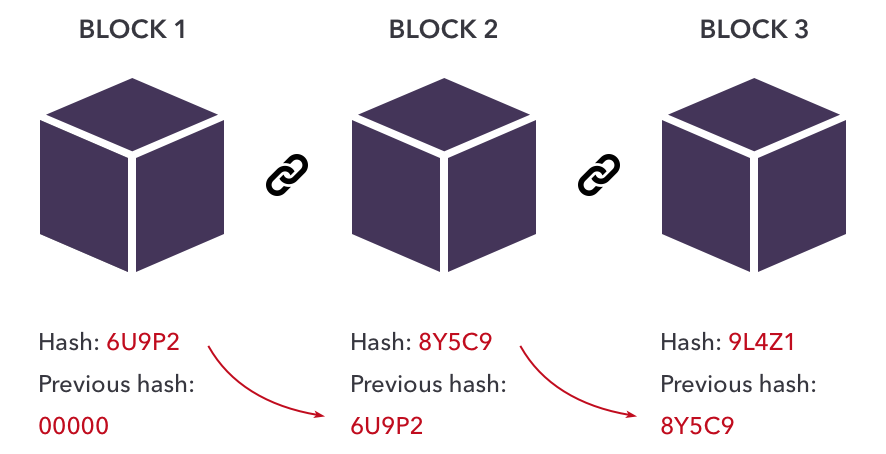
\includegraphics[width=10cm]{images/chapter1/blockchain.png}
		\caption{{\footnotesize Abstract Blockchain blocks visualization}}
\end{figure}

A Blockchain network can track orders, payments, accounts, production and much more. And because members of the network share a single view of the truth, you can see all details of a transaction end to end, giving you greater confidence, as well as new efficiencies and opportunities.\newpage

\section{Problem \& motivation}

Elections are expensive, complicated to set up and even on extreme cases fraudulent. This democratic system is almost 3000 years old and it has not evolved since ancient Greece. It entails an obligation for the voters to rely on third party officials and groups to safely collect votes and publish results, In the case of the modern democratic nation of France for example, there are only 3000 magistrates delegated to supervise and monitor more than 35 000 communes\cite{republiquefrancaiseArticleLO274Code2021}, a feat that is inconceivable for them to physically achieve, so setting the human malice apart still leaves room for human error, both leading to the voters carrying justifiable suspicions to any result the ballot may yield. Classic elections also carry hefty financial burdens, the 43rd general election (December 31st, 2020) of Canada had a total estimated cost of \$502.4 million\cite{electionscanadaEstimatedCost43rd2021}, the equivalent of the cost of building 5 new hospitals, including administrative areas, operating and emergency rooms, and space for 120 beds\cite{fixrcompanyCostBuildHospital2020}.

\begin{wrapfigure}[13]{r}{5cm}
	\vspace{-10pt}
	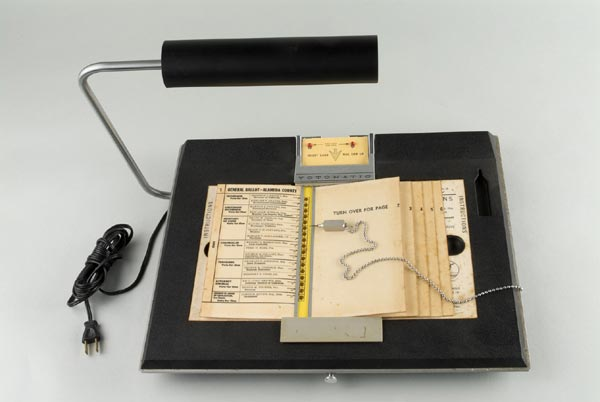
\includegraphics[width=5cm]{images/chapter1/votomatic.jpg}
	\vspace{-10pt}
	\caption{{\footnotesize The Votomatic vote recorder, a punch card voting machine originally developed in the mid 1960s}}
	\label{votomatic}
\end{wrapfigure}

Then comes technology, the premise held while entering various fields is that it will increase efficiency, cut costs and leave all parties involved satisfied, with an abundance of examples of when technology did also keep that premise, voting seems to be a logical place to land in next. Electronic voting systems and semi-electronic ones existed for quite some time, from punched card systems {\small (see figure \ref{votomatic})} to modern-day digital voting machines. However, they only served to optimize the physical act of punching a card or putting a piece of enveloped paper in a box, although that did cut some costs, may be made the experience of voting more pleasant, but it introduced more security concerns and most importantly it did not solve the essential problem of eliminating third parties, because people still had to trust the hardware and software engineers that programmed the machines to cast the votes, and the servers to not allow for any tampering with the data.\newpage


\section{Purpose \& delimitations}
The goal of this work is to investigate the possibility of using the new surging Blockchain technology as the underlying technology powering an electronic voting system, offering the ability to store the results in a decentralized ledger that should grant the solution attributes like immutability and transparency. We intend to achieve our goal by designing a decentralized e-voting system as a \gls{proof-of-concept}, capable of launching an election, casting votes and displaying results, all while ensuring transparency, anonymity, security and above all correctness of the results.
It is of major importance to define the scope of this work document and its underlying implementation.

First, the implementation of the proof of concept is not by any means complete and thorough but instead functionality was compromised in favor of delivering an actual election on the Blockchain.

Second, regarding Blockchain technology, this document will not dive deep into the inner workings of the technology, topics like hash functions, cryptography and proof of work mechanism will not be presented in a manner that debates their efficiency since we judge the scientific literature on these subjects to be of abundance, the focus will instead fall on how the application of this technology on voting would look like.

\vspace{2cm}

\begin{figure}[h]
	\centering
		
\includegraphics[width=3cm]{images/chapter1/verum.png}
		\caption{{\footnotesize Proof-of-concept "Verum" Logo}}
\end{figure}\newpage

\section{Document structure}
This document is presented in 5 chapters, starting with the chapter 1: Introduction, in which we present a bit of background of the topic and then delve into formally defining the problem we intend to tackle, followed by a brief description of what lies within and beyond the scope of this work.

In Chapter 2: Technical background, we present sufficient technical background about the two major aspects of our project, being the Ethereum Blockchain and Web applications. The next chapter, Chapter 3: Contribution \& system design. Next comes chapter 4: Implementation, a chaper about the implementation of our proof-of-concept, in which tools are introduced and results are displayed using diagrams, screenshots and language.

Finally, in chapter 5: Conculusion and prespectives, the results and insights gained through the journey of making our proof-of-concept are discussed, few conclusions drawn and perspectives on what could be enhanced moving forward with this project.
\chapter{Technical background}
This chapter presents an overview of the technical concepts involved in the realization of this project, namely the Ethereum Blockchain and Web applications
\section{Ethereum Blockchain}
Ethereum is a blockchain platform with its own \gls{cryptocurrency}, called Ether (ETH) or Ethereum, and its own programming language, called Solidity. As a blockchain network, Ethereum is a decentralized public ledger for verifying and recording transactions. The network's users can create, publish, monetize, and use applications on the platform, and use its Ether cryptocurrency as payment. Insiders call the decentralized applications on the network "dapps."

\begin{wrapfigure}[10]{r}{4cm}
	\vspace{-10pt}
	
\includegraphics[width=4cm]{images/chapter2/ethereum.png}
	\vspace{-10pt}
	\caption{{\footnotesize Ethereum Blockchain logo}}
\end{wrapfigure}

Ethereum intends to create an alternative protocol for building decentralized applications, providing a different set of tradeoffs that its creators believe will be very useful for a large class of decentralized applications, with particular emphasis on situations where rapid development time, security for small and rarely used applications, and the ability of different applications to very efficiently interact, are important. Ethereum does this by building what is essentially the ultimate abstract foundational layer: a blockchain with a built-in Turing-complete programming language, allowing anyone to write smart contracts and decentralized applications where they can create their own arbitrary rules for ownership, transaction formats and state transition functions.

In the Ethereum universe, there is a single, canonical computer (called the Ethereum Virtual Machine, or \acrshort{EVM}) whose state everyone on the Ethereum network agrees on. Everyone who participates in the Ethereum network (every Ethereum node) keeps a copy of the state of this computer. Additionally, any participant can broadcast a request for this computer to perform arbitrary computation. Whenever such a request is broadcast, other participants on the network verify, validate, and carry out ("execute") the computation. This causes a state change in the EVM, which is committed and propagated throughout the entire network.

\subsection{Accounts}
In Ethereum, the state is made up of objects called "accounts", with each account having a 20-byte address and state transitions being direct transfers of value and information between accounts. An Ethereum account contains four fields:

\begin{itemize}
\item The \textbf{nonce}, a counter used to make sure each transaction can only be processed once
\item The account's current \textbf{ether} balance
\item The account's \textbf{contract code}, if present
\item The account's \textbf{storage} (empty by default)
\end{itemize}

"Ether" is the main internal crypto-fuel of Ethereum, and is used to pay transaction fees. In general, there are two types of accounts: \textbf{externally owned accounts}, controlled by private keys, and \textbf{contract accounts}, controlled by their contract code. An externally owned account has no code, and one can send messages from an externally owned account by creating and signing a transaction; in a contract account, every time the contract account receives a message its code activates, allowing it to read and write to internal storage and send other messages or create contracts in turn.\newpage

\begin{figure}[h]
	\centering
		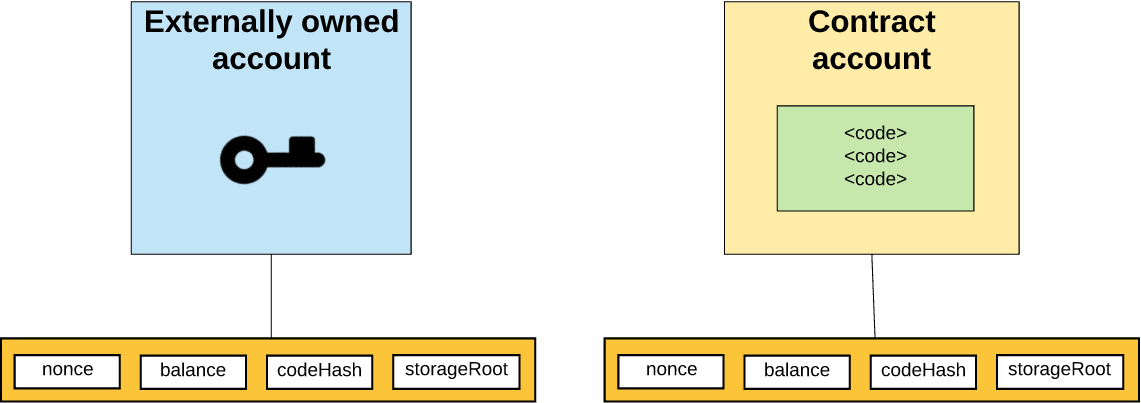
\includegraphics[width=10cm]{images/chapter2/accounts.png}
		\caption{{\footnotesize Abstract Ethereum accounts visualization}}
\end{figure}

\subsection{Transactions}
An Ethereum transaction refers to an action initiated by an externally-owned account, in other words an account managed by a human, not a contract. For example, if Bob sends Alice 1 ETH, Bob's account must be debited and Alice's must be credited. This state-changing action takes place within a transaction.

\begin{figure}[H]
	\centering
		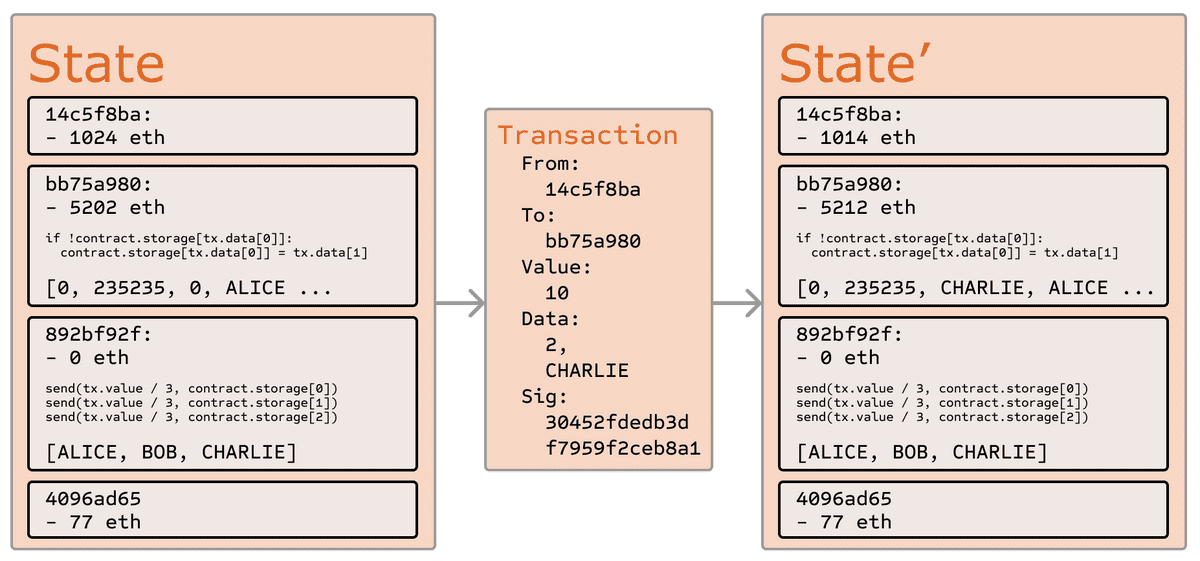
\includegraphics[width=10cm]{images/chapter2/transition.png}
		\caption{{\footnotesize Abstract representation of an Ethereum transaction}}
\end{figure}

Transactions, which change the state of the EVM, need to be broadcast to the whole network. Any node can broadcast a request for a transaction to be executed on the EVM; after this happens, a miner will execute the transaction and propagate the resulting state change to the rest of the network.

Transactions require a fee and must be mined to become valid. To make this overview simpler we'll cover gas fees and mining elsewhere.

A submitted transaction includes the following information:

\begin{itemize}
\item \textbf{recipient} - the receiving address (if an externally-owned account, the transaction will transfer value. If a contract account, the transaction will execute the contract code)
\item \textbf{signature} - the identifier of the sender. This is generated when the sender's private key signs the transaction and confirms the sender has authorised this transaction
\item \textbf{value} - amount of ETH to transfer from sender to recipient (in WEI, a denomination of ETH)
\item \textbf{data} - optional field to include arbitrary data
\item \textbf{gasLimit} - the maximum amount of gas units that can be consumed by the transaction. Units of gas represent computational steps
\item \textbf{gasPrice} - the fee the sender pays per unit of gas
\end{itemize}

Gas is a reference to the computation required to process the transaction by a miner. Users have to pay a fee for this computation. The gasLimit and gasPrice determine the maximum transaction fee paid to the miner (more on gas on later subsections.

\subsection{Gas}
Gas refers to the unit that measures the amount of computational effort required to execute specific operations on the Ethereum network.

Since each Ethereum transaction requires computational resources to execute, each transaction requires a fee. Gas refers to the fee required to successfully conduct a transaction on Ethereum.

\begin{figure}[h]
	\centering
		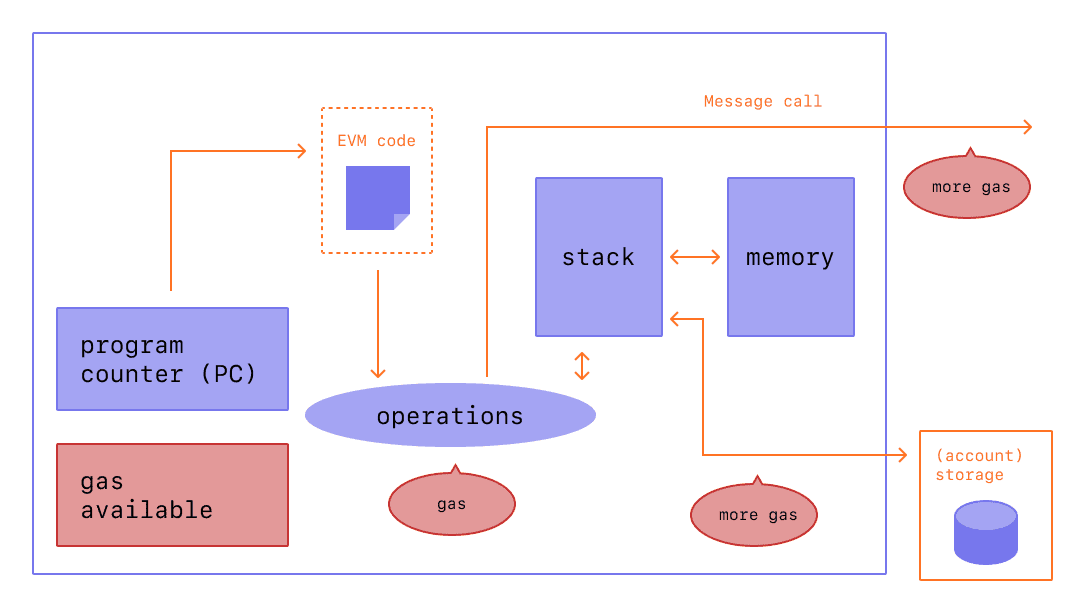
\includegraphics[width=10cm]{images/chapter2/gas.png}
		\caption{{\footnotesize Diagram of the role of gas in Ethereum \cite{TakenobuhsEthereumevmillustratedEthereum}}}
\end{figure}

In essence, gas fees are paid in Ethereum's native currency, ether (ETH). Gas prices are denoted in gwei, which itself is a denomination of ETH - each gwei is equal to 0.000000001 ETH (10-9 ETH). For example, instead of saying that your gas costs 0.000000001 ether, you can say your gas costs 1 gwei.

Gas fees exist because they help keep the Ethereum network secure. By requiring a fee for every computation executed on the network, we prevent actors from spamming the network. In order to prevent accidental or hostile infinite loops or other computational wastage in code, each transaction is required to set a limit to how many computational steps of code execution it can use. The fundamental unit of computation is "gas".

\subsection{Consensus mechanisms}
When it comes to blockchains like Ethereum, which are in essence distributed databases, the nodes of the network must be able to reach agreement on the current state of the system. This is achieved using consensus mechanisms.

Consensus mechanisms (also known as consensus protocols or consensus algorithms) allow distributed systems (networks of computers) to work together and stay secure.

For decades, these mechanisms have been used to establish consensus among database nodes, application servers, and other enterprise infrastructure. In recent years, new consensus protocols have been invented to allow \gls{cryptoeconomic} systems, such as Ethereum, to agree on the state of the network.

A consensus mechanism in a cryptoeconomic system also helps prevent certain kinds of economic attacks. In theory, an attacker can compromise consensus by controlling 51\% of the network. Consensus mechanisms are designed to make this "\gls{51attack}" unfeasible. Different mechanisms are engineered to solve this security problem differently.
\subsubsection{Types of consensus mechanisms}

\begin{description}
\item[Proof of work] Proof-of-work is done by miners, who compete to create new blocks full of processed transactions. The winner shares the new block with the rest of the network and earns some freshly minted \gls{ETH}. The race is won by whoever's computer can solve a math puzzle fastest – this produces the cryptographic link between the current block and the block that went before. Solving this puzzle is the work in "proof of work".
\item[Proof of stake] Proof-of-stake is done by validators who have staked ETH to participate in the system. A validator is chosen at random to create new blocks, share them with the network and earn rewards. Instead of needing to do intense computational work, you simply need to have staked your ETH in the network. This is what incentivises healthy network behaviour.
\end{description}

\subsection{Dapps}

A dapp has its backend code running on a decentralized peer-to-peer network. Contrast this with an app where the backend code is running on centralized servers.

A dapp can have frontend code and user interfaces written in any language (just like an app) that can make calls to its backend. Furthermore, its frontend can be hosted on decentralized storage.

\begin{description}
\item[Decentralized] means they are independent, and no one can control them as a group.
\item[Deterministic] they perform the same function irrespective of the environment they are executed.
\item[Turing complete] which means given the required resources, the dapp can perform any action.
\item[Isolated] which means they are executed in a virtual environment known as Ethereum Virtual Machine so that if the smart contract happens to have a bug, it won’t hamper the normal functioning of the blockchain network.
\end{description}

\begin{figure}[H]
	\centering
		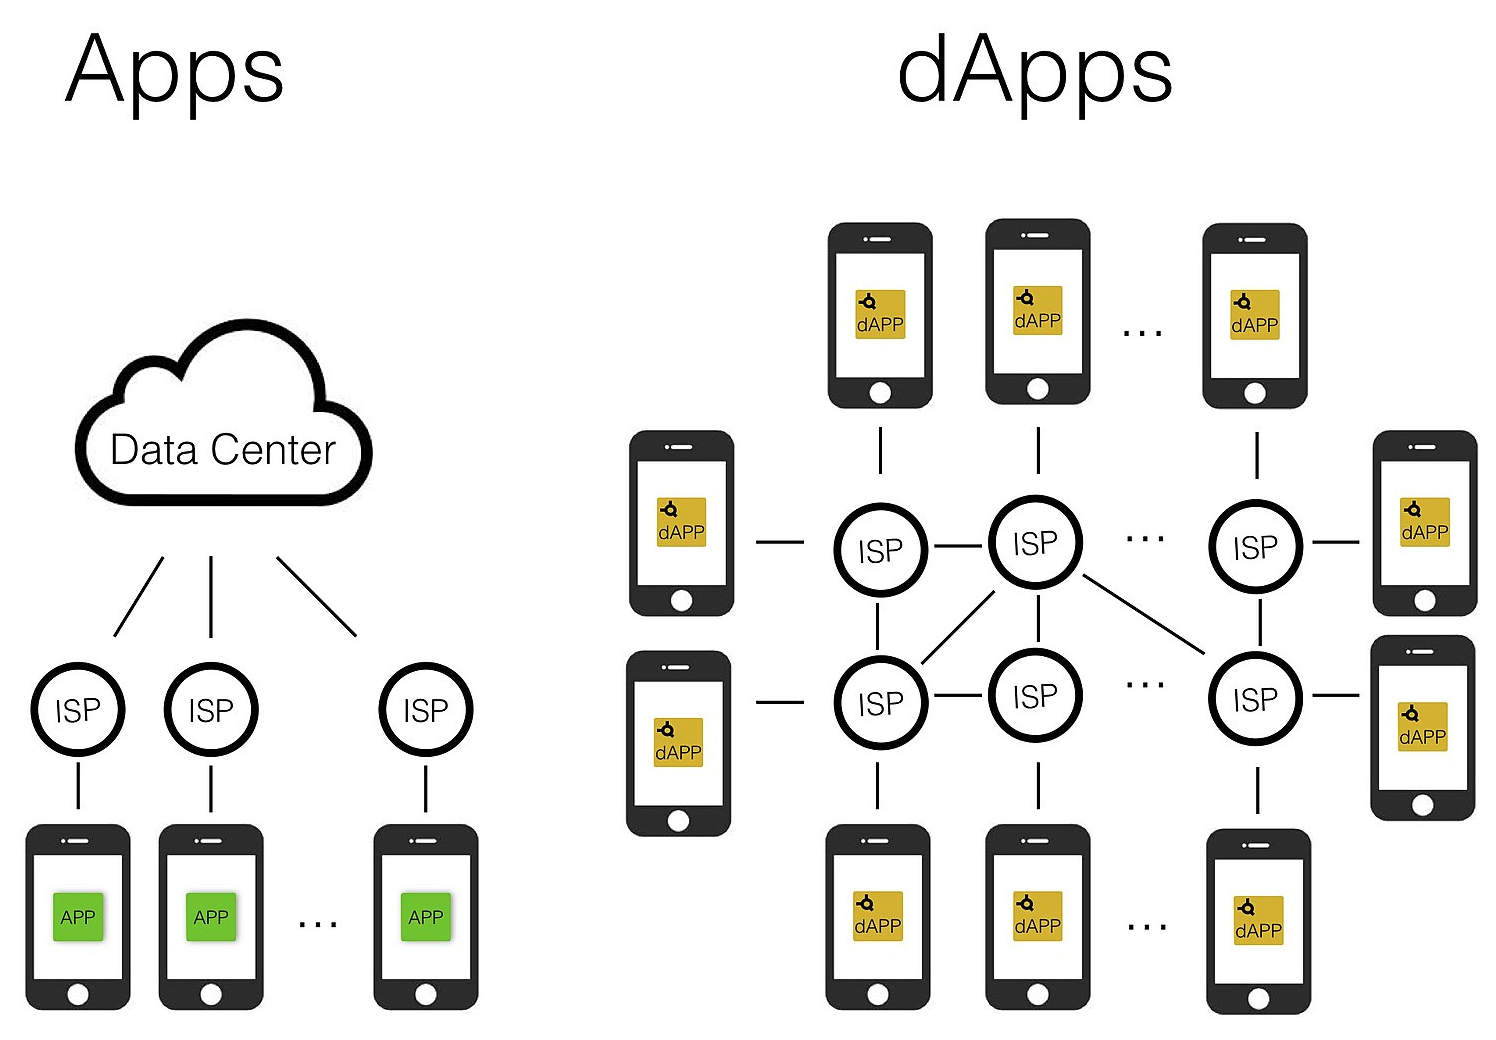
\includegraphics[width=10cm]{images/chapter2/dapps.png}
		\caption{{\footnotesize Diagram of centralized and decentralized applications topology}}
\end{figure}

\subsection{Smart contracts}

A smart contract is simply put a program that runs on the Ethereum blockchain. It's a collection of code (its functions) and data (its state) that resides at a specific address on the Ethereum blockchain.They runs exactly as programmed. Once they are deployed on the network they can't be changed. Dapps can be decentralized because they are controlled by the logic written into the contract, not an individual or company.

Smart contracts are a type of Ethereum account. This means they have a balance and they can send transactions over the network. User accounts can then interact with a smart contract by submitting transactions that execute a function defined on the smart contract. Smart contracts can define rules, like a regular contract, and automatically enforce them via the code.\medskip

Ethereum has developer-friendly languages for writing smart contracts:

\begin{itemize}
\item Solidity
\item Vyper 
\end{itemize}

\section{Web Applications}

A web application (or web app) is application software that runs on a web server, unlike computer-based software programs that are run locally on the operating system (OS) of the device. Web applications are accessed by the user through a web browser with an active network connection. These applications are programmed using a client–server modeled structure—the user ("client") is provided services through an off-site server that is hosted by a third-party. Examples of commonly-used web applications include: web-mail, online retail sales, online banking, and online auctions.

\subsection{Structure}

Applications are usually broken into logical chunks called "tiers", where every tier is assigned a role. Traditional applications consist only of 1 tier, which resides on the client machine, but web applications lend themselves to an n-tiered approach by nature.[3] Though many variations are possible, the most common structure is the three-tiered application.\cite{MakeNtierArchitecture} In its most common form, the three tiers are called presentation, application and storage, in this order. A web browser is the first tier (presentation), an engine using some dynamic Web content technology (such as ASP, CGI, ColdFusion, Dart, JSP/Java, Node.js, PHP, Python or Ruby on Rails) is the middle tier (application logic), and a database is the third tier (storage). The web browser sends requests to the middle tier, which services them by making queries and updates against the database and generates a user interface.

For more complex applications, a 3-tier solution may fall short, and it may be beneficial to use an n-tiered approach, where the greatest benefit is breaking the business logic, which resides on the application tier, into a more fine-grained model.\cite{MakeNtierArchitecture} Another benefit may be adding an integration tier that separates the data tier from the rest of tiers by providing an easy-to-use interface to access the data. For example, the client data would be accessed by calling a "list\_clients()" function instead of making an SQL query directly against the client table on the database. This allows the underlying database to be replaced without making any change to the other tiers.

There are some who view a web application as a two-tier architecture. This can be a "smart" client that performs all the work and queries a "dumb" server, or a "dumb" client that relies on a "smart" server. The client would handle the presentation tier, the server would have the database (storage tier), and the business logic (application tier) would be on one of them or on both.\cite{MakeNtierArchitecture} While this increases the scalability of the applications and separates the display and the database, it still doesn't allow for true specialization of layers, so most applications will outgrow this model.

\subsection{Business use}

An emerging strategy for application software companies is to provide web access to software previously distributed as local applications. Depending on the type of application, it may require the development of an entirely different browser-based interface, or merely adapting an existing application to use different presentation technology. These programs allow the user to pay a monthly or yearly fee for use of a software application without having to install it on a local hard drive. A company which follows this strategy is known as an application service provider (ASP), and ASPs are currently receiving much attention in the software industry.

Security breaches on these kinds of applications are a major concern because it can involve both enterprise information and private customer data. Protecting these assets is an important part of any web application and there are some key operational areas that must be included in the development process. This includes processes for authentication, authorization, asset handling, input, and logging and auditing. Building security into the applications from the beginning can be more effective and less disruptive in the long run.

Cloud computing model web applications are software as a service (SaaS). There are business applications provided as SaaS for enterprises for a fixed or usage-dependent fee. Other web applications are offered free of charge, often generating income from advertisements shown in web application interface\cite{TopTipsSecure}.

\subsection{Development}

Writing web applications is often simplified by the use of web application framework. These frameworks facilitate rapid application development by allowing a development team to focus on the parts of their application which are unique to their goals without having to resolve common development issues such as user management. Many of the frameworks in use are open-source software.

The use of web application frameworks can often reduce the number of errors in a program, both by making the code simpler, and by allowing one team to concentrate on the framework while another focuses on a specified use case. In applications which are exposed to constant hacking attempts on the Internet, security-related problems can be caused by errors in the program. Frameworks can also promote the use of best practices such as GET after POST.

In addition, there is potential for the development of applications on Internet operating systems, although currently there are not many viable platforms that fit this model\cite{FrameworkDocForgeProgramming}.
%\chapter{Implementation}

In this chapter, the process of implementation will be covered, starting by the architecture and the tools to the results and how everything fits together.

\section{Architecture}
\section{Tools}
\subsection{React JS}

\begin{wrapfigure}[10]{r}{3cm}
	\vspace{-10pt}
	
\includegraphics[width=3cm]{images/chapter3/logo-react-js.png}
	\vspace{-10pt}
	\caption{{\footnotesize React JS framework logo}}
\end{wrapfigure}

React (also known as React.js or ReactJS) is a free and open-source front-end JavaScript library\cite{ReactJavaScriptLibrary} for building user interfaces or UI components. It is maintained by Facebook and a community of individual developers and companies.\cite{ReactMakingFaster} React can be used as a base in the development of single-page or mobile applications. However, React is only concerned with state management and rendering that state to the DOM, so creating React applications usually requires the use of additional libraries for routing, as well as certain client-side functionality.

\subsection{Web3.js}

There are a few different aspects to developing blockchain applications with Ethereum:

\begin{itemize}
\item \textbf{Smart contract development} - writing code that gets deployed to the blockchain with the Solidity programming language.
\item \textbf{Developing websites or clients that interact with the blockchain} - writing code that reads and writes data from the blockchain with smart contracts.
\end{itemize}

\begin{wrapfigure}[9]{r}{3cm}
	\vspace{-10pt}
	
\includegraphics[width=3cm]{images/chapter3/web3.jpeg}
	\vspace{-10pt}
	\caption{{\footnotesize Web3 logo}}
\end{wrapfigure}

Web3.js enables you to fulfill the second responsibility: developing clients that interact with The Etherem Blockchain. It is a collection of libraries that allow you to perform actions like send Ether from one account to another, read and write data from smart contracts, create smart contracts, and so much more.

Web3.js communicates to The Ethereum Blockchain with JSON RPC, which stands for "Remote Procedure Call" protocol. Ethereum is a peer-to-peer network of nodes that stores a copy of all the data and code on the blockchain. Web3.js allows us to make requests to an individual Ethereum node with JSON RPC in order to read and write data to the network\cite{mccubbinIntroWeb3Js}.

\subsection{Ganache}

\begin{wrapfigure}[11]{r}{2.5cm}
	\vspace{-10pt}
	
\includegraphics[width=2.5cm]{images/chapter3/ganache-logo-dark.png}
	\vspace{-10pt}
	\caption{{\footnotesize Ganache Logo}}
\end{wrapfigure}

Ganache is a personal blockchain for rapid Ethereum and Corda distributed application development. You can use Ganache across the entire development cycle; enabling you to develop, deploy, and test your dApps in a safe and deterministic environment.

Ganache comes in two flavors: a UI and CLI. Ganache UI is a desktop application supporting both Ethereum and Corda technology. The command-line tool, ganache-cli (formerly known as the TestRPC), is available for Ethereum development. Prefer using the command-line? This documentation will focus only on the UI flavor of Ganache. Please see the Ganache CLI Readme for command-line documentation.

All versions of Ganache are available for Windows, Mac, and Linux\cite{GanacheOverviewDocumentation}.

\begin{figure}[H]
	\centering
		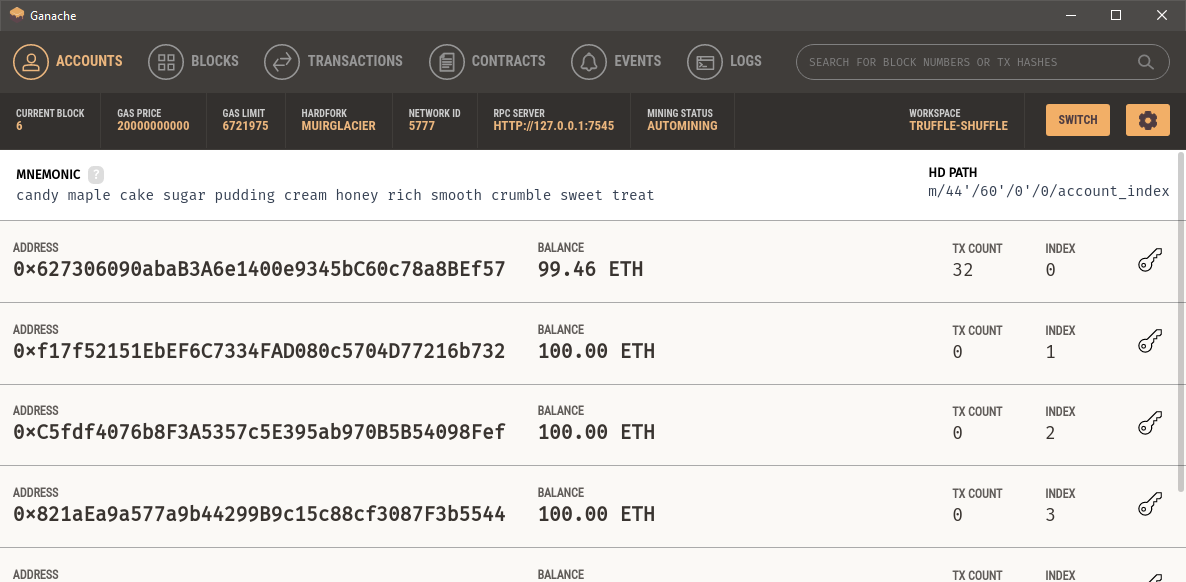
\includegraphics[width=10cm]{images/chapter3/ganache-window.png}
		\caption{{\footnotesize Ganache GUI}}
\end{figure}

\subsection{MetaMask}

\begin{wrapfigure}[10]{r}{2.5cm}
	\vspace{-10pt}
	
\includegraphics[width=2.5cm]{images/chapter3/metamask-logo.png}
	\vspace{-10pt}
	\caption{{\footnotesize MetaMask Logo}}
\end{wrapfigure}

MetaMask is a software cryptocurrency wallet used to interact with the Ethereum blockchain.\cite{schroederCryptoWalletMetaMask2020} It allows users to access their Ethereum wallet through a browser extension or mobile app, which can then be used to interact with decentralized applications.

MetaMask allows users to store and manage account keys, broadcast transactions, send and receive Ethereum-based cryptocurrencies and tokens, and securely connect to decentralized applications through a compatible web browser or the mobile app's built-in browser.[3][4]

The application includes an integrated service for exchanging Ethereum tokens by aggregating several decentralized exchanges (DEXs) to find the best exchange rate. This feature, branded as MetaMask Swaps, charges a service fee of 0.875\% of the transaction amount\cite{schroederCryptoWalletMetaMask2021}.

\begin{figure}[h]
	\centering
		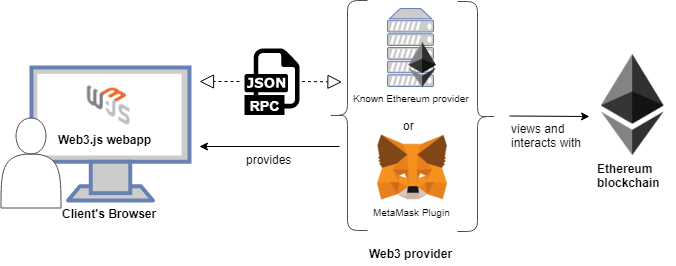
\includegraphics[width=10cm]{images/chapter3/web3-architecture.png}
		\caption{{\footnotesize architecture of a client application interaction with a blockchain network using Web3 and MetaMask}}
\end{figure}

\section{Results}
\subsection{Admin dashboard}
\subsection{End-user (voter) application}
\subsection{Authentication}
\subsection{Smart contract}
%\chapter{Conclusion \& perspectives}

The idea of adapting digital voting systems to make electoral processes cheaper, faster and easier, is a compelling one in modern society. Making the electoral process cheap and quick, normalizes it in the eyes of the voters, removes a certain power barrier between the voter and authorities. It also opens the door for developing countries to aspire for better democracy.

In our work, we introduced a unique, blockchain-based electronic voting system by building a proof-of-concept that utilizes smart contracts to enable secure and cost efficient election while guaranteeing transparency and integrity. We have outlined the systems architecture, the design, and a visual demonstration of what it would look like. Essential trade-offs had to be made along the way, for example introducing a complementary backend server that serves the purpose of cutting the storing of data on the Blockchain costs significantly, however it also exposes the system to DDoS attacks that can target the authentication phase of the voting and jeopardize the whole election. One possible solution to remedy that particular issue would be the use of local databases on the voting machines and performing authentication locally on each machine, that would not eliminate all the risks, however it would ensure that the election can't be stopped by malicious third parties.

Ethereum Blockchain technology as it stands today suffers various shortcomings, the technology is vastly criticized for its outrageous energy consumption and carbon footprint, to put it in perspective a typical Ethereum transaction gobbles more power than an average U.S. household uses in a day\cite{fairleyEthereumWillCut2019}, but the Ethereum founders and community are promising a more scalable, more secure and more sustainable version of the technology that they're calling Ethereum 2.0, it uses 1\% of the energy it uses today to complete transactions\cite{fairleyEthereumWillCut2019}.

For the future, it will be interesting to see how the upgrades on Ethereum could impact this particular application of the technology, or will there ever be a new Blockchain implementation tailored specifically for elections.

Our system design and prototype remain to be tested on real Ethereum \gls{testnets} and further optimize our system.


\bibliographystyle{plain}
\bibliography{bibliography}
%
%\input{Parts/resume.tex}

\end{document}
